	\subsection{Analog interface board}
	A smaller part of the hardware design is an analog board with two function: It has to convert the signal from the current transducers and the torque sensor into a analog signal between $0V$ and $1V$ for ADC's.
	
	\subsubsection{Current transducer}
	The current transducer used in this project is the LF 205-S. This transducer has the conversion ratio $1:2000$, this means when the maximum current, $\pm 300A$, passes through, it will give a signal between $\pm 50mA$. This $\pm 50mA$ has to be converted into a $\pm 0.5V$ signal. That is achieved by using a shunt resistor, which is calculated to be:
	
	\begin{equation}
		R = \frac{0.5V}{50mA} = 3.33\Omega
	\end{equation}
	
	This resistance is made by setting three $10 \Omega$ in parallel.

	Now the signal from the current transducer is converted to be between $\pm 0.5V$. This has to be offset by $+0.5V$, resulting in a signal varying between $0$ and $1V$. This is done using a 'AD620A', which is an instrumentation amplifier with an offset input. The two $R_g$ port on the 'AD620A' is going to be left open, which will give a unity gain on the output.
	
	\begin{figure}[H]
		\centering
		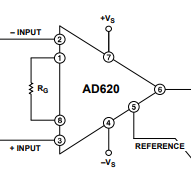
\includegraphics[width=0.4\textwidth]{pictures/hardware/Analog_Interface_board/AD620A.PNG}
		\caption{Instrumentation amplifier AD620A}
		\label{fig:AD620A}
	\end{figure} 
	
	The input reference to the 'AD620A' has to be very exact. Small differences can cause great inaccuracies in the current measuring. Therefore a voltage reference is used to keep a stable voltage at $0.5V$. The used voltage reference, a LM385Z-1.2 in conjunction with a voltage divider of resistors $R1 = 1k\ohm$, $R2 = 1k\ohm$, $R3 = 470\ohm$ yields a constant voltage of
	
	\begin{equation}
		V = V_{ref} \cdot \frac{R1}{R1+R2+R3} = 0.5V
	\end{equation}
	
	where 
	
	\begin{equation}
	V_{ref} = 1.235V
	\end{equation}
	
	A Buffer is added to give a low impedance signal to the 'AD620A'.
	
	At the input of the Instrumentation amplifier a resistor is placed at both the inverting and the non-inverting input to reduce current. Using the AD620A is also advantageous for its high CMRR (Common-mode Rejection ratio) that helps with cancelling out noise present on both input pins with the same waveform. It can also use the $\pm15V$ dual supply present on the board.
	
	\subsubsection{Torque pedal measurement}
	The output of the torque pedal connects to the same ADC as one of the current channels, hence it also has to be in the range of $0-1V$. The pedal is basically a $7.5k\ohm$ potmeter, so the idea is to parallel it with the lower resistor of a voltage divider to get about $1V$ at full range. Using $V_{ref_3} = 3.3V$ as excitation for the divider and $R1 = R2 = 10K\ohm$, the following equation is true at full throttle: 
	
	\begin{equation}
		V = V_{ref_3} \cdot \frac{R_{pot} \times R15}{R_{pot} \times R15 + R14} = 0.99V
	\end{equation}
	
	When the pedal is not pressed at all, the $0\ohm$ of the potmeter shunts the supply to the ground.
	
	\begin{figure}[H]
	\centering
	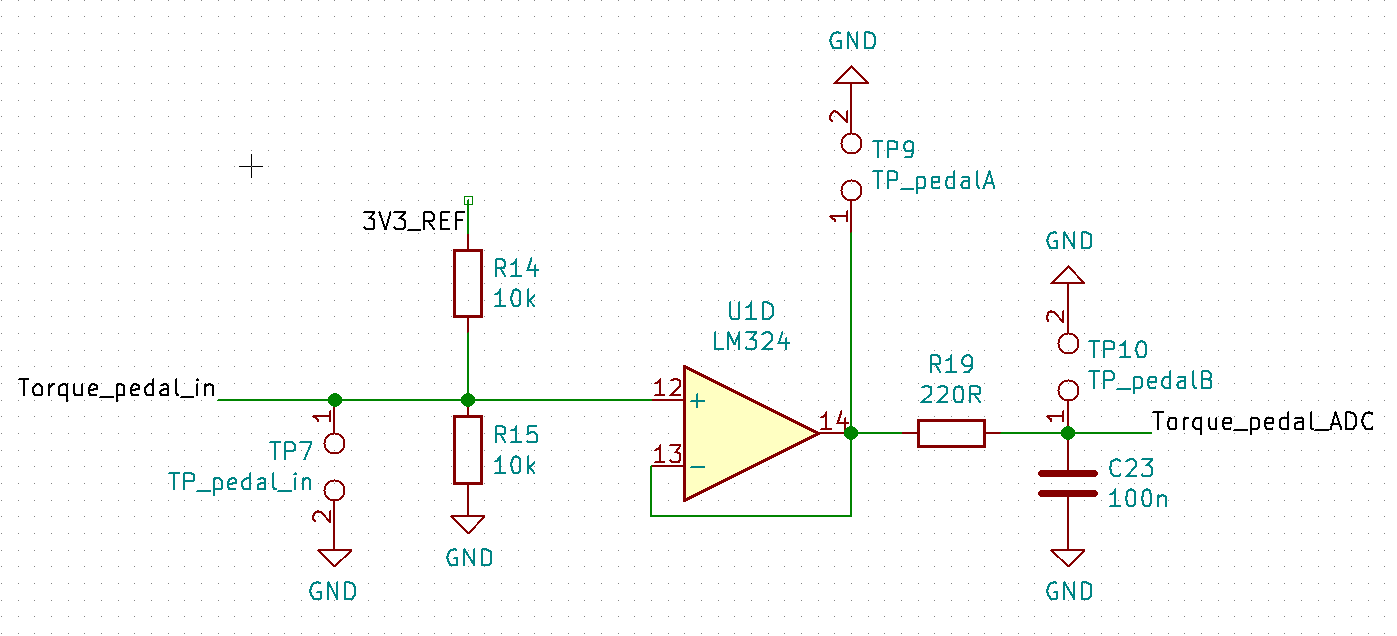
\includegraphics[width=0.6\linewidth]{pictures/hardware/Analog_Interface_board/torque_pedal_divider.png}
	\caption{Torque pedal reading circuit}
	\label{fig:torque_pedal_divider}
\end{figure}
	
	For this channel, an opamp in voltage follower configuration is sufficient instead of an instrument amplifier, since no offsetting is required.